%!TEX root = ../thesis.tex
\chapter{The one with data and BOW\label{ch:dataandBOW}}

The main source of data for analysis is draw from the Twitter accounts of news-media organisations. In the 1950s, the widespread popularity of household television allowed TV broadcasting to become the primary tool for influencing public opinion in developed nations~\todo{cite: Diggs-Brown, Barbara (2011) Strategic Public Relations: Audience Focused Practice p.48}.  This was a shift from a population that \emph{listened} to radio news, to a population that \emph{watched} news. 

The even more rapid rise of mobile internet and social media sites in the last two decades has caused another shift. No longer just a population that watch news at fixed time, or read regularly scheduled newspapers; the conveniences of the modern developed world allow individuals to consume news anytime, anywhere. As of 2019, 55\% of US adults get their news from social media either `often' or `sometimes'~ and 88\% state that `social media companies have at least some control over the mix of news people see'~'\cite{shearerAmericansAreWary2019}.

Given the importance of a free press and the role of social media sites in the delivery of news, this work aims to study the news on social media. To begin this task, we first define some common terms for clarity.

\begin{definition}[Social media]
	The platforms used to consume information by individuals in the public. E.g. Twitter, Facebook, Reddit.
\end{definition}

\begin{definition}[News-media]
	The organisations that are producing information about a broad range of current events and sharing that information with the public.
\end{definition}

\begin{definition}[News]
	The \emph{content} produced by news-media organisations. 
\end{definition}

\section{Data}

% <allsides disscussion>
Using the media analysis source AllSides\footnote{www.allsides.com}, a collection of news-media organisations was found. The purpose of AllSides is to provide an open  analysis of political leanings of news sources~\tocite{ https://www.allsides.com/media-bias/media-bias-ratings}, and to aggregate news allowing consumers to view articles from different sides of the political spectrum. Each news source is labelled into one of 5 categories, Left, Lean Left, Center, Lean Right, or Right. Any news source the ratings are determined internally using `blind surveys of people across the political spectrum, multi-partisan analysis, editorial reviews, third party data, and tens of thousands of user feedback ratings'~\tocite{same as above}. News sources are only assigned to a single category, but do have an attached confidence rating that is provided from users selecting if they agree or disagree with the rating. An example of the ratings can be seen in \autoref{fig:allsidesmediabiaschart}.

\begin{figure}
	\centering
	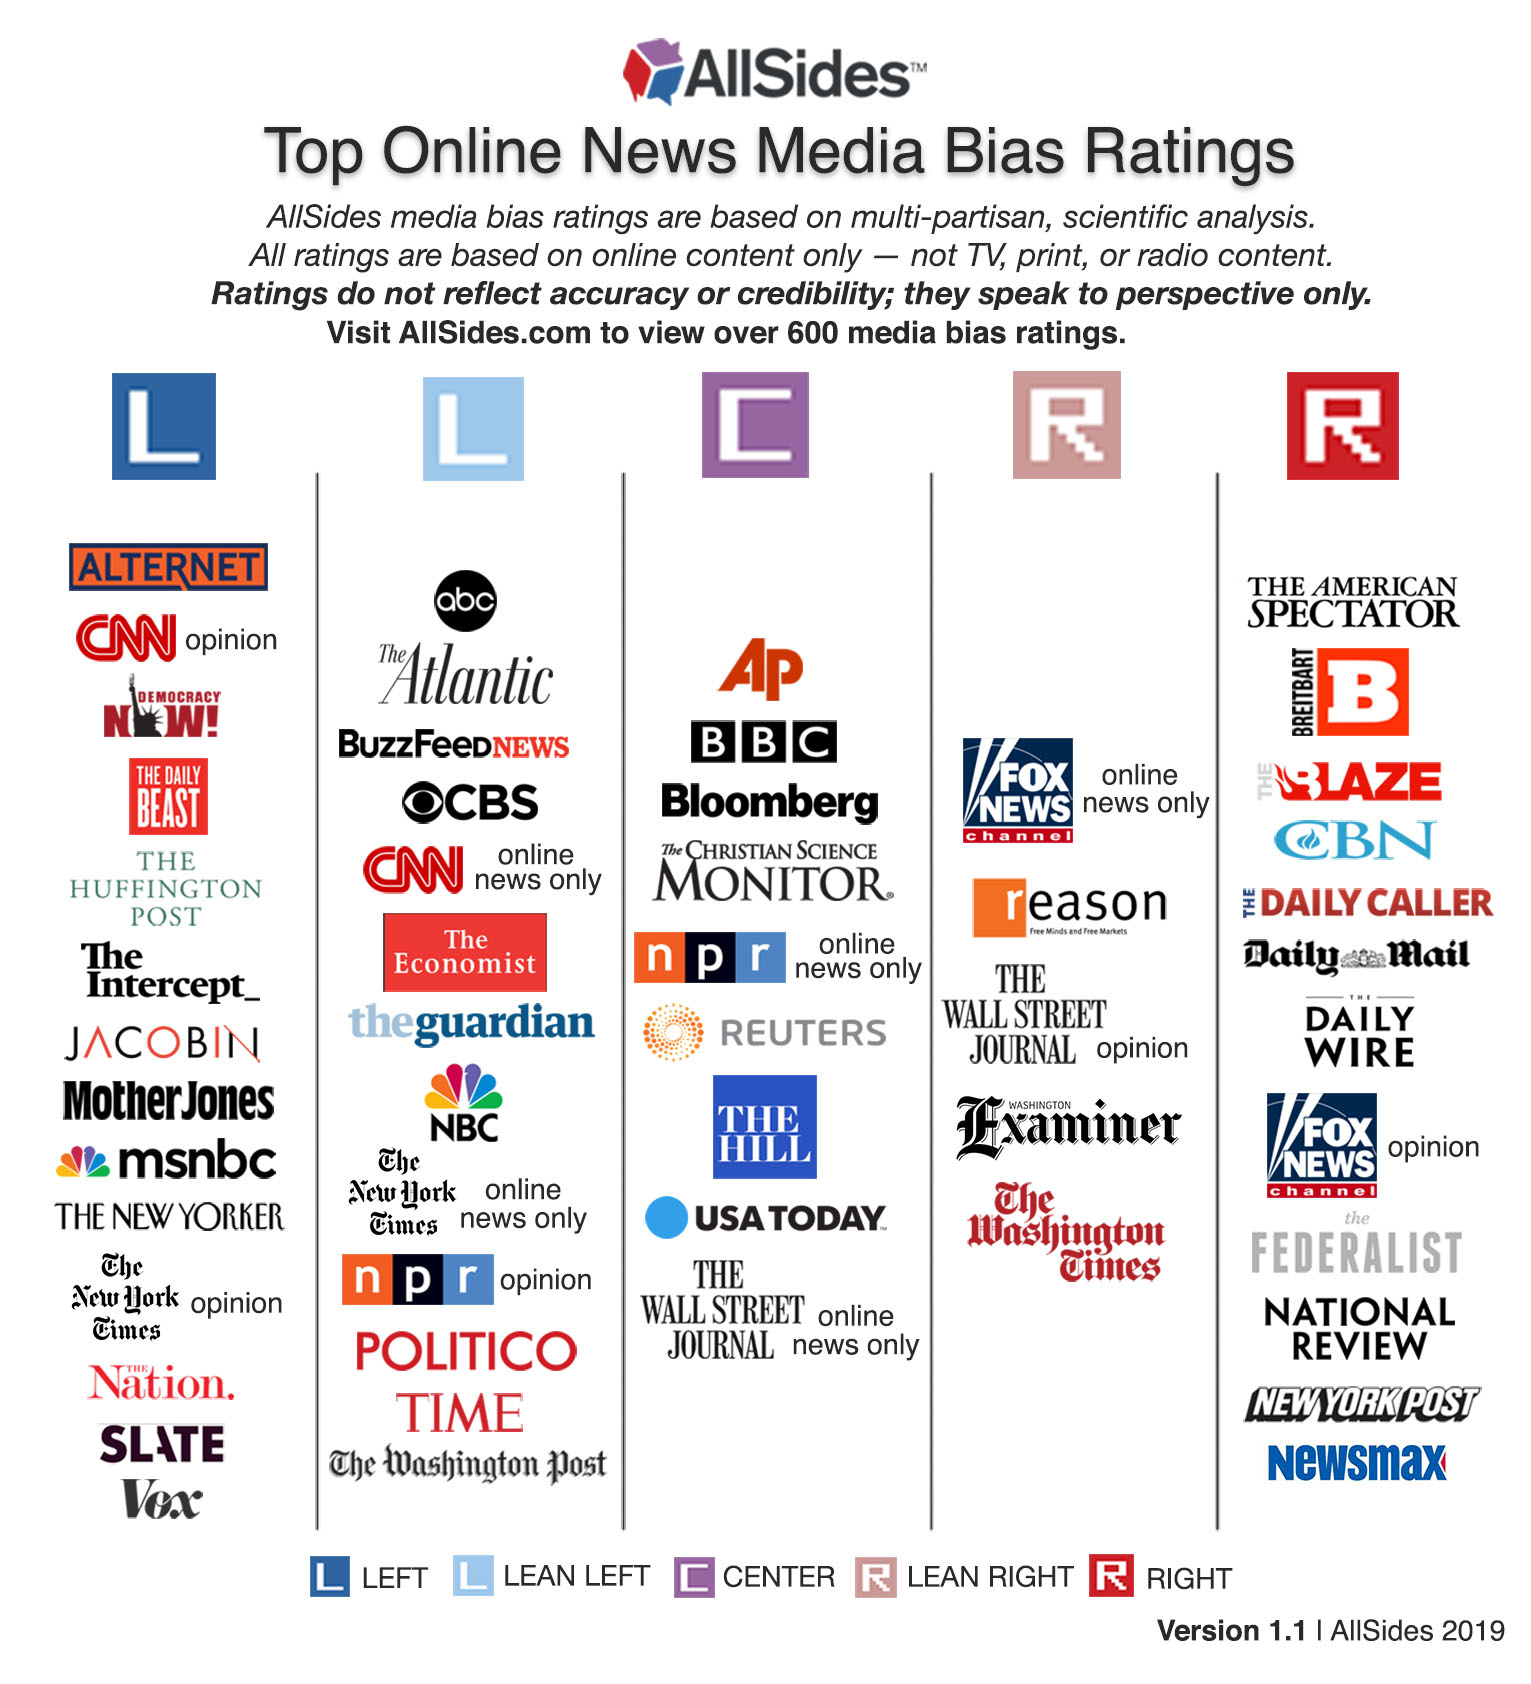
\includegraphics[width=0.9\linewidth]{chapter1/figs/AllSidesMediaBiasChart}
	\caption{An example collection of News-Media sites that have been classified into biases by AllSides; sourced from \tocite{https://www.allsides.com/media-bias/media-bias-ratings (as above)}}
	\label{fig:allsidesmediabiaschart}
\end{figure}




% </allsides disscussion>

%  <twitter collection>
From the website, a list of possible news sources was collected on February 1st, 2019. In this collection was organisation names, political bias', the number of user feedback ratings of the political bias, and, if available, the twitter handles associated with those sources. These collected news sources were broad, containing not just news-media organisations but authors, pundits and think tanks. 

To select an appropriate set of news-media organisation an examination and filtering process was undertaken. A source was only considered if it was a organisation (not an individual), that produced news content of a diverse range of topics. Many news sources were connected to think tanks or opinion groups, and only created news of a single topic or campaign. Further, if an news-media organisation has no twitter account or had less than 10,000 followers (a low bar in the social media world), then it was removed from the pool. This mainly removed inactive organisations and news organisation from small rural towns. Finally, a single source was removed as it was not in English, and a single source was removed as it was the smaller sister site that had all content as a subset of it's larger site.  The result of this filtering process is 174 news-media organisations and associated twitter accounts and categorised political bias'.  A list of all news-media organisations under analysis can be seen in \cite{app:accounts} and all removed sources and the removal justification can be seen in \todo{appendix of removals}.

%twitter collection
Using the Twitter user handles associated with each of the news-media organisations, the history of all tweets for each account was collected using the Twitter application programming interface (API)\footnote{https://developer.twitter.com/en/docs} and web-scraping tools~\tocite{twint}. Of interest in this work are the tweets each news organisation tweeted between January 1st, 2019 to January 1st, 2020. 

% removal of inactive twitter accounts
Using this collection method a total of 3,221,769 tweets were collected from the 174 news-media organisation official Twitter accounts. 

% average twitter activity
% plots of the daily twitter activities of each news organition of 
52.97 tweets per day





%  filtering and why we removed them



As a result of this filtering we are left with 154 news-media organisations with complete data for the 2019 calendar year. Of these organisations the bias distribution is still somewhat representative of social media. \todo{find a source that discusses why left wing is more popular on social media.} In total there are 73 organisations in the left half of the bias spectrum, 44 in the centre and 37 on the right; expanded on in \autoref{fig:numberofbiasorganisations}. This distribution, although shifted towards the left, still provides ample sources for the effect of bias to be explored further in this work, with keen attention to the potential impact of the skewed distribution. 

\begin{table}[h]
	\begin{tabular}{lr}
		\toprule
		Bias &   Number of Organisations \\
		\midrule
		{\color{Left} Left }&  31 \\
		{\color{LeanLeft} Lean Left }&  42 \\
		{\color{Center} Center }&  44 \\
		{\color{LeanRight} Lean Right }&  16 \\
		{\color{Right} Right }&  21 \\
		\bottomrule
	\end{tabular}
	\caption{The number of news-media organisation in each political bias classification within our data.}
	\label{fig:numberofbiasorganisations}
\end{table}


% <metadata>
From the news-media Twitter accounts we can also access metadata about the organisation. Two useful such pieces of metadata are the geographic location ,as determined to be posted by the organisation, and the number of followers on twitter.

% location diverstity but america

% follower distributions (by bias?)


% somewhere
60054638 words
